\documentclass[11pt,a4paper]{report}

\usepackage[utf8]{inputenc}
\usepackage{graphicx}
\usepackage{caption}
\usepackage{subcaption}
\usepackage{listings}
\usepackage[nottoc]{tocbibind}
\usepackage[bottom]{footmisc}
\usepackage{todonotes}
\usepackage[hidelinks]{hyperref}

\graphicspath{{resources/images/}}

\lstset{basicstyle = \ttfamily,
        columns = fullflexible,
        keepspaces = true,
        backgroundcolor = \color{lightgray},
        showstringspaces = false,
        upquote = true,
        breaklines = true,
}

\begin{document}
    \hypersetup{pageanchor=false}
    \begin{titlepage}
        \begin{center}
            \textsc{\LARGE Bachelor thesis\\Computing Science}\\[1.5cm]
            
\includegraphics[height=100pt]{logo}

            \vspace{0.4cm}
            \textsc{\Large Radboud University}\\[1cm]
            \hrule
            \vspace{0.4cm}
            \textbf{\huge Creating a Methodology for Penetration Testing of Docker Containers}\\[0.4cm]
            \hrule
            \vspace{2cm}
            \begin{minipage}[t]{0.45\textwidth}
                \begin{flushleft} \large
                    \textit{Author:}\\
                    Joren Vrancken\\
                    s4593847
                \end{flushleft}
            \end{minipage}
            \begin{minipage}[t]{0.45\textwidth}
                \begin{flushright} \large
                    \textit{Supervisor:}\\
                    Associate professor, Erik Poll\\
                    \texttt{erikpoll@cs.ru.nl}\\[1.3cm]
                    \textit{Internship supervisor:}\\
                    Dave Wurtz\\
                    \texttt{dave.wurtz@secura.com}\\[1.3cm]
                    \textit{Second internship supervisor:}\\
                    Geert Smelt\\
                    \texttt{geert.smelt@secura.com}
                \end{flushright}
            \end{minipage}

            \vfill {\large \today}
            \hfill

            \todo[inline]{TODOs are shown like this.}
        \end{center}
    \end{titlepage}

    \begin{abstract}
Containerization software has become extremely popular to streamline software deployments in the last few years. That has made it a very import attack surface. This paper looks at how one should go about testing the security of the Docker containers. It first looks at known vulnerabilities and misconfigurations that impact the security. It links those to the Docker CIS Benchmark (security guidelines). It then provides a methodology for Secura to test the security of Dockers in the networks of their clients.
\end{abstract}

    \hypersetup{pageanchor=true}

    \tableofcontents

    \chapter{Introduction}
\todo[inline]{Not about app vulnerabilities, but specifically about Docker}
\todo[inline]{Docker is not a security framework}
\todo[inline]{What is the added security value of Docker?}

Secura, a company specializing in digital security, performs security assessments for clients. In these assessments, Secura evaluates vulnerable parts of the private and public network of their clients. They would like to improve those assessments by also looking into containerization software their clients may be running.

\hfill

Containerization software allows developers to package software into easily reproducible packages.
It removes the tedious process of installing the right dependencies to run software, because the dependencies and necessary files are neatly isolated in the container. This also allows multiple versions of the same software to run simultaneous on a server, because every instance runs in its own container.

The de facto industry standard is called Docker. Docker allows developers to package software into images and run those instances as containers.

Docker streamlines and significantly simplifies software development and deployment. That is why many companies use Docker to develop, test and deploy (part of) their IT infrastructure someway or another. This makes it very interesting from a security perspective. A security problem with Docker could have a large impact on organizations.

\hfill

This research paper describes possible security problems with Docker (vulnerabilities and misconfigurations) and how those can be used during security assessments.

    \chapter{Background}\label{chapter:background}

In this chapter we will discuss the necessary background information and preliminaries. First we will look at what containerization software is and how it compares to virtualization. We will also look at important Docker concepts, how to use them and how Docker works internally. Finally, we introduce the CIS Docker Benchmarks.

\section{Containerization Software}\label{background:containerization}
\todo[inline]{Jos: Better models with examples}
Containerization software isolates processes running on a host from each other.
A process in a container sees a different part of the host system than processes outside of the container. A process inside a container sees a different file system, network interfaces and users than processes outside of the container. Processes inside the container can only see other processes inside the container.

\begin{figure}[ht]
    \centering
    \begin{subfigure}[t]{.45\textwidth}
        \centering
        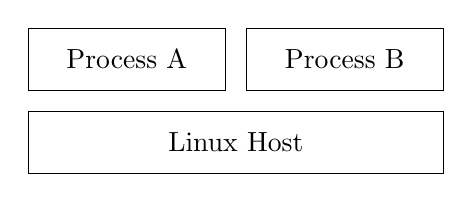
\begin{tikzpicture}[x=0.75pt,y=0.75pt,yscale=-1,xscale=1]
            % Process A Rectangle
            \draw (0,25) -- (95,25) -- (95,55) -- (0,55) -- cycle ;
            \draw (47.5,40) node {Process A};

            % Process B Rectangle
            \draw (105,25) -- (200,25) -- (200,55) -- (105,55) -- cycle ;
            \draw (152.5,40) node {Process B};

            % Host Rectangle
            \draw (0,65) -- (200,65) -- (200,95) -- (0,95) -- cycle ;
            \draw (100, 80) node {Linux Host};
        \end{tikzpicture}
        \caption{Two processes.}\label{subfig:processes}
    \end{subfigure}
    \begin{subfigure}[t]{.45\textwidth}
        \centering
        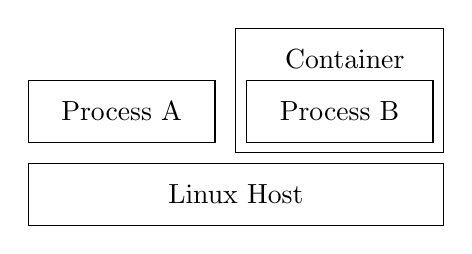
\begin{tikzpicture}[x=0.75pt,y=0.75pt,yscale=-1,xscale=1]
            % Process A Rectangle
            \draw (0,25) -- (90,25) -- (90,55) -- (0,55) -- cycle ;
            \draw (45,40) node {Process A};

            % Process B container Rectangle
            \draw (100,0) -- (200,0) -- (200,60) -- (100,60) -- cycle ;
            \draw (152.5,15) node {Container};

            %% Process B Rectangle
            \draw (105,25) -- (195,25) -- (195,55) -- (105,55) -- cycle ;
            \draw (150,40) node {Process B};

            % Host Rectangle
            \draw (0,65) -- (200,65) -- (200,95) -- (0,95) -- cycle ;
            \draw (100, 80) node {Linux Host};
        \end{tikzpicture}
        \caption{One process in a container.}\label{subfig:container}
    \end{subfigure}
    \caption{}\label{fig:with-without-container}
\end{figure}

If we look at \autoref{fig:with-without-container}, we see two scenarios. \autoref{subfig:processes} is the normal way to run processes. The operating system starts processes that can communicate with other processes. Their view on the file system is the same.
In \autoref{subfig:container} one of the processes runs inside a container. These processes cannot communicate with one another. If Process A looks at the files in \lstinline{/tmp}, it accesses a different part of the file system than when Process B looks at the files in \lstinline{/tmp}\footnote{Access to files on the host has to be explicitly given (as discussed in \autoref{subsection:data-persistence}).}. Process B can not even see that Process A exists.

\medskip

Process A and Process B see such a different part of the host system that to Process B it looks like it is running on a wholly different system.

\subsection{Advantages of Containerization}
\todo[inline]{Jos: better explanation}
Containers can be made into easily deployable packages (called images). These images only contain the necessary files for specific software to run. Other files, libraries and binaries are shared between the host operating system (the system running the container). This allows developers to create lightweight software packages containing only the necessary dependencies.

\medskip

Containers also make it possible to run multiple versions of the same software on one host. Each container can contain a specific version and all the containers run on the same host. Because the containers are isolated from each other, their incompatible dependencies do not pose a problem.

\medskip

For example, if we want to run an instance of Wordpress\footnote{A very popular content management system to build websites with.}, we do not need to install all the Wordpress dependencies. We only need to download the container that the Wordpress developers created, which includes all the necessary dependencies.

Similarly, if we want to move the Wordpress instance from one host to another, we just have to copy the Wordpress database and run the image on the new host. Even if the new host is a completely different operating system.

If we want to test a newer version of Wordpress on the same host, we only have to run the different container on the same host. The incompatible dependencies of the two Wordpress instances are not a problem, because they see different parts of the file system and do not even see each other's processes.

\medskip

The simplicity that containerization brings, makes containerization very popular in software development, maintenance and deployment.

\pagebreak

\subsection{Virtualization}
\todo[inline]{Jos: Hypervisior separate from host in image}
Virtualization is an older, similar technique to isolate software. In virtualization, a whole system is simulated on top of the host (called the hypervisor). This new virtual machine is called a guest. The guest and the host do not share any system resources. This has some advantages. For example, it allows running a completely different guest operating system (e.g.\ a Windows guest on a Linux host).

\begin{figure}[ht]
    \centering
    \begin{subfigure}[t]{.45\textwidth}
        \centering
        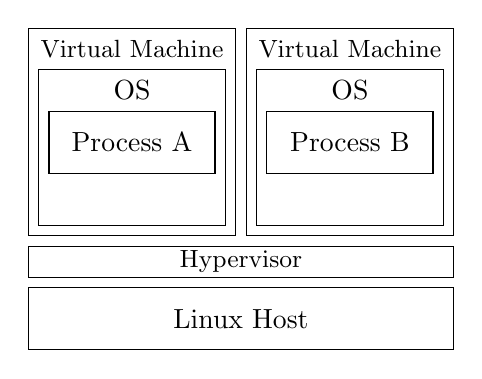
\begin{tikzpicture}[x=0.75pt,y=0.75pt,yscale=-1,xscale=1]
            % VM Process A Rectangle
            \draw (0,0) -- (100,0) -- (100,100) -- (0,100) -- cycle ;
            \draw (50,10) node {{\small Virtual Machine}};

            % OS Process A Rectangle
            \draw (5,20) -- (95,20) -- (95,95) -- (5,95) -- cycle ;
            \draw (50,30) node {OS};

            % Process A Rectangle
            \draw (10,40) -- (90,40) -- (90,70) -- (10,70) -- cycle ;
            \draw (50,55) node {Process A};

            % VM Process B Rectangle
            \draw (105,0) -- (205,0) -- (205,100) -- (105,100) -- cycle ;
            \draw (155,10) node {{\small Virtual Machine}};

            % OS Process B Rectangle
            \draw (110,20) -- (200,20) -- (200,95) -- (110,95) -- cycle ;
            \draw (155,30) node {OS};

            % Process B Rectangle
            \draw (115,40) -- (195,40) -- (195,70) -- (115,70) -- cycle ;
            \draw (155,55) node {Process B};

            % Hypervisor
            \draw (0,105) -- (205,105) -- (205,120) -- (0,120) -- cycle ;
            \draw (102.5,112.5) node {{\small Hypervisor}};

            % Linux Host
            \draw (0,125) -- (205,125) -- (205,155) -- (0,155) -- cycle ;
            \draw (102.5,140) node {Linux Host};
        \end{tikzpicture}
        \caption{Virtual Machines\protect\footnotemark.}
    \end{subfigure}
    \begin{subfigure}[t]{.45\textwidth}
        \centering
         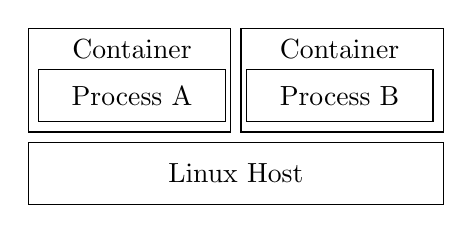
\begin{tikzpicture}[x=0.75pt,y=0.75pt,yscale=-1,xscale=1]
            % Container Process A Rectangle
            \draw (0,0) -- (97.5,0) -- (97.5,50) -- (0,50) -- cycle ;
            \draw (50,10) node {Container};

            % Process A Rectangle
            \draw (5,20) -- (95,20) -- (95,45) -- (5,45) -- cycle ;
            \draw (50,32.5) node {Process A};

            % Container Process B Rectangle
            \draw (102.5,0) -- (200,0) -- (200,50) -- (102.5,50) -- cycle ;
            \draw (150,10) node {Container};

            % Process B Rectangle
            \draw (105,20) -- (195,20) -- (195,45) -- (105,45) -- cycle ;
            \draw (150,32.5) node {Process B};

            % Host Rectangle
            \draw (0,55) -- (200,55) -- (200,85) -- (0,85) -- cycle ;
            \draw (100, 70) node {Linux Host};
        \end{tikzpicture}
        \caption{Containers.}
    \end{subfigure}
    \caption{}
\end{figure}
\footnotetext{Hypervisors can also run on the bare metal. This removes the need for a host OS, which adds security.}

Because containerization software shares many resources with the host, it is a lot faster and more flexible than virtualization. Where virtualization needs to start a whole new operating system, containerization only needs to start a single process.

\subsection{The Impact of Containers on Security}
\todo[inline]{Jos: explain RCE}
A Docker container isolates software from the host, but does not change it. This means that vulnerabilities in software are not affected by Dockerizing that software. However, the impact of those vulnerabilities is decreased, because the vulnerability exists in an isolated environment.

If, for example, there exists a remote code execution (RCE) vulnerability in Wordpress. Running Wordpress in a Docker container does not fix the vulnerability. An attacker is still able to exploit it. But the attacker is far less likely to access the host system, because the exploited software is isolated from the host system because of Docker.

\medskip

Because a container uses the same kernel and resources as the host, a \lstinline{root} exploit (i.e.\ an exploit that allows unprivileged users to escalate their privileges) can be just as effective inside as outside of the container, because the target (e.g.\ the kernel) is the same. CVE--2016--5195(Dirty Cow)\footnote{\url{https://dirtycow.ninja/}} is a good example of an exploit that allows container escapes\cite{Dirty-Cow-Escape}, because it attacks the kernel of the host.

\section{Docker}
\todo[inline]{Docker on Windows}
\todo[inline]{Research: Secure Computing Mode Profiles}
\todo[inline]{\href{https://itnext.io/chroot-cgroups-and-namespaces-an-overview-37124d995e3d}{chroot, cgroups and namespaces}}
\todo[inline]{\href{https://www.secura.com/blog-hacklu2018-docker-security}{Docker, A brief history and security considerations for modern environments}}

\hfill

The concept of containerization has been around a long time, but it only gained traction as serious way to package, distribute and run software in the last few years. This is mostly because of Docker.

\hfill

Docker was released in 2013 and it did not only offer a containerization platform, but also a way to distribute the containers. This allows developers and companies to create packages that are much more easily run.

\hfill

For example, someone that wants to run an instance of Wordpress\footnote{A very popular content management system to build websites with.}, does not need to install all the Wordpress dependencies. They only need to download the Docker image that the Wordpress developers created.
Similarly, if they want to move the Wordpress instance from one host to the other, they just have to copy over their database and run the Docker image on the new host. Even if the new host is a completely different operating system.

\subsection{Docker Concepts}
Docker is based on four concepts: Docker daemon, Docker images, Docker containers and \lstinline{Dockerfile}s.

\subsubsection{Docker daemon}
The daemon is a service that runs on the host machine. It manages all things related to Docker on that machine. For example if the user wants to build an image or a container needs to restart the docker daemon. It is good to note that, because everything related to Docker is handled by the daemon and Docker has access to all resources of the host, having access to Docker should be viewed as equivalent to having \lstinline{root} access to the host\footnote{\url{https://docs.docker.com/engine/security/security/\#docker-daemon-attack-surface}}.

\subsubsection{Docker images}
A Docker image is packaged software. It is a distributable set of layers. The first layer describes the base of the image. This is either an existing image or nothing (referred to as \lstinline{scratch}). Each layer on top of that is a change to the layer before. For example, if you add a file or run an command it adds a new layer.

\subsubsection{Docker containers}
A container is an instance of a Docker Image. If you run software packaged as a Docker image, you create a container based on that image. If you want to run two instances of the same Docker image, you can create two containers.

\subsubsection{\lstinline{Dockerfile}s}
A \lstinline{Dockerfile} describes what a Docker image is made of. It describes the steps to build the image. Lets look at a very simple example:

\begin{lstlisting}[caption={Very Basic \lstinline{Dockerfile}},label={dockerfile:simple},captionpos=b]
FROM alpine:latest
LABEL maintainer="Joren Vrancken"
CMD ["echo", "Hello World"]
\end{lstlisting}

These three instructions tell the Docker engine how to create a new Docker image.
The full instructionset can be found in the \lstinline{Dockerfile} reference\footnote{\url{https://docs.docker.com/engine/reference/builder/}}

\begin{enumerate}
    \item The \lstinline{FROM} instruction tells the Docker engine what to base the new Docker image on. Instead of creating an image from scratch (a blank image), we use an already existing image as our basis.

    \item The \lstinline{LABEL} instruction sets a key value pair for the image. There can be multiple LABEL instructions. These key value pairs get packaged and distributed with the image.

    \item The \lstinline{CMD} instruction sets the default command that should be run and which arguments should be passed to it.
\end{enumerate}

We can use this to create a new image and container from that image.
\begin{lstlisting}[caption={Creating a Docker container from a \lstinline{Dockerfile}},label={docker:container},captionpos=b]
$ docker build -t thesis-hello-world .
$ docker run --rm --name=thesis-hello-world-container thesis-hello-world
\end{lstlisting}

We first create a Docker image (called \lstinline{thesis-hello-world}) using the \lstinline{docker build} command and then create and start a new container (called \lstinline{thesis-hello-world-container}) from that image.

\subsubsection{Data Persistence}
Without additional configuration, a Docker container does not have persistence storage. Its storage is maintained when the container is stopped, but not when the container is removed.

\subsubsection{Networking}
\todo[inline]{iptables}
\todo[inline]{\url{https://github.com/docker/libnetwork/blob/master/docs/design.md}}

When a Docker container is created Docker creates a network sandbox for that container and (by default) connects it to an internal bridge network. This gives the container its own networking resources such as a IPv4 address\footnote{IPv6 support is not enabled by default.}, routes and DNS entries. All outgoing traffic is routed through a bridge interface (by default).

\hfill

Incoming traffic is possible by routing traffic for specific ports from the host to the container.
Specifying which ports on the host are routed to which ports on the container is done when a container is created. If we, for example, want to expose port \lstinline{80} to the Docker image created from the \hyperref[dockerfile:simple]{first \lstinline{Dockerfile}} we can execute the following commands.

\begin{lstlisting}[caption={Creating a Docker container with exposed port},label={docker:publish},captionpos=b]
$ docker build -t thesis-hello-world .
$ docker run --rm --publish 8000:80 --name=thesis-hello-world-container thesis-hello-world
\end{lstlisting}

The first command creates a Docker image using the \lstinline{Dockerfile} and we then create (and start) a container from that image. We ``publish'' port \lstinline{8000} on the host to port \lstinline{80} of the container. This means that, while the container is running, all traffic from port \lstinline{8000} on the host is routed to port \lstinline{80} of the container.

\subsubsection{Docker internals}
\todo[inline]{\href{https://medium.com/@saschagrunert/demystifying-containers-part-i-kernel-space-2c53d6979504}{Demystifying Containers Part I Kernel Space}}
\todo[inline]{\href{https://medium.com/@saschagrunert/demystifying-containers-part-ii-container-runtimes-e363aa378f25}{Demystifying Containers Part II Container Runtimes}}
\todo[inline]{\href{https://medium.com/@saschagrunert/demystifying-containers-part-iii-container-images-244865de6fef}{Demystifying Containers Part III Container Images}}

\subsection{docker-compose}
\todo[inline]{Secrets in docker-compose can be easily found, even without docker group permissions}

\subsection{Registries}
\todo[inline]{Official images not always standard images}

Docker images are distributable through so called registries. A registry is a server (that anybody can host), that stores Docker images. When a client does not have a Docker image that it needs, it can contact a registry to download that image.

\hfill

The most popular (and public) registry is Docker Hub, which is run by company that develops Docker.
Anybody can create a Docker Hub account and start creating images that anybody can download. Docker Hub also provides default images for popular software.

\section{CIS Docker Benchmarks}
The Center for Internet Security (or CIS for short) is a non-profit organization that provides best practice solutions for digital security. For example, they provide security hardened virtual machine images that are configured for optimal security.

\hfill

The CIS Benchmarks are guidelines and best practices on security on many different types of software. These guidelines are freely available for anyone and can be found on their site\footnote{\url{https://cisecurity.org/cis-benchmarks/}}. Many companies (e.g. Secura) use the CIS Benchmarks as a baseline to assess the security of systems.

\hfill

They also provide guidelines on Docker\footnote{Only Docker CE, the community edition. It does not cover Docker EE, the enterprise edition.}. The latest version (1.2.0) contains 115 guidelines. These are sorted by topic (e.g. Docker daemon and configuration files). In \hyperref[appendix:CIS-Benchmark-Example]{the appendix} you will find an example guideline from the latest Docker CIS Benchmark.


    \chapter{Known vulnerabilities in Docker}

\todo[inline]{Map this chapter to CIS Docker Benchmark}
\todo[inline]{\href{https://resources.whitesourcesoftware.com/blog-whitesource/top-5-docker-vulnerabilities}{Top 5 Docker Vulnerabilities You Should Know}}
\todo[inline]{\href{https://neoteric.eu/blog/docker-containers-with-root-privileges/}{Docker containers with root privileges}}
\todo[inline]{\url{https://www.katacoda.com/courses/docker-security/}}
\todo[inline]{\href{https://media.ccc.de/v/Camp2019-10178-hacking_containers_and_kubernetes}{Hacking Containers and Kubernetes}}

\section{Vulnerabilities}
\section{Misconfigurations}
\todo[inline]{Permissions on config/service files}
\todo[inline]{Wrong volumes: / or /proc}
\todo[inline]{Non-docker group Docker access?}
\todo[inline]{Research: create user and group in Dockerfile}

    \chapter{Penetration Testing of Docker}\label{chapter:pentesting}
In \autoref{chapter:vulnerabilities-misconfigurations} we looked at specific attacker models, individual vulnerabilities and individual misconfigurations. In this chapter we will look at how we would use those during a penetration test. We will first look at how to use them manually. After that, we will look at how we can automate the manual steps.

\hfill

We will mostly focus on the misconfigurations, because although the vulnerabilities might have a high impact they are all mitigated with one line of advice: ``Keep your systems up to date''.

\section{Manual}
\todo[inline]{Which attack scenarios from 3 are relevant?}

\subsection{Attack Context Detection}
\todo[inline]{Detect running in a Docker}
\todo[inline]{Detect Docker (running) on host}
\todo[inline]{\href{https://github.com/rapid7/metasploit-framework/blob/master/modules/post/linux/gather/checkcontainer.rb}{Metasploit Linux Gather Container Detection}}

\subsection{Testing from Host}
\todo[inline]{What images are available on the host?}
\todo[inline]{systemctl cat docker}
\todo[inline]{/etc/default/docker}
\todo[inline]{daemon.json}
\todo[inline]{firewall rules}
\todo[inline]{docker binary setuid}
\todo[inline]{check if docker is installed}
\todo[inline]{check docker socket}
\todo[inline]{Which users are in the docker group}
\todo[inline]{Open ports to Docker socket?}
\todo[inline]{What containers are running}
\todo[inline]{Docker version, does not require docker permissions}

\subsection{Testing from Container}
\todo[inline]{\href{https://stackoverflow.com/questions/32144575/how-to-know-if-a-docker-container-is-running-in-privileged-mode}{How to know if a docker container is running in privileged mode}}
\todo[inline]{grep Cap /proc/1/status}
\todo[inline]{capsh --decode=00000000a80425fb}
\todo[inline]{Reachable containers}
\todo[inline]{ARP Spoofing other containers}
\todo[inline]{Privileged capability 0000003fffffffff}
\todo[inline]{find docker socket}
\todo[inline]{Identify host OS and container OS}
\todo[inline]{root in container}

\section{Automated}
\todo[inline]{\href{https://github.com/ProfessionallyEvil/harpoon}{harpoon}}
\todo[inline]{Source \href{https://www.zenko.io/blog/5-free-tools-to-navigate-through-docker-containers-security}{5-free-tools-to-navigate-through-docker-containers-security}}
\todo[inline]{Static analysis tool: \url{https://github.com/coreos/clair}}
\todo[inline]{Scanner for clair: \url{https://github.com/arminc/clair-scanner}}
\todo[inline]{Static vulnerability scanner (and clamAV) on software in container: \url{https://github.com/eliasgranderubio/dagda}}
\todo[inline]{\href{https://github.com/goodwithtech/dockle}{Dockle}}
\todo[inline]{Scanner using the CIS Docker Benchmark: \url{https://github.com/docker/docker-bench-security}}
\todo[inline]{SaaS container policy scanner: \url{https://anchore.com}}
\todo[inline]{Research: Twistlock}
\todo[inline]{Research: Sqreen}
\todo[inline]{sysdig: \url{https://sysdig.com/}}
\todo[inline]{sysdig: \url{https://sysdig.com/opensource/falco/}}

    \chapter{Future Work}
\section{Kubernetes}
\todo[inline]{Kubernetes Pod Escape Using Log Mounts: \url{https://blog.aquasec.com/kubernetes-security-pod-escape-log-mounts}}
\todo[inline]{Container Platform Security at Cruise: \url{https://medium.com/cruise/container-platform-security-7a3057a27663}}
\todo[inline]{\href{https://hub.packtpub.com/an-unpatched-security-issue-in-the-kubernetes-api-is-vulnerable-to-a-billion-laughs-attack/}{An unpatched security issue in the Kubernetes API is vulnerable to a ``billion laughs'' attack}}
\todo[inline]{\href{https://itnext.io/learn-about-the-basics-of-kubernetes-persistence-part-1-b1fa2847768f}{Basics of Kubernetes Volumes (Part 1)}}
\todo[inline]{\href{https://itnext.io/tutorial-basics-of-kubernetes-volumes-part-2-b2ea6f397402}{Basics of Kubernetes Volumes (Part 2)}}
\todo[inline]{What is the added value of virtualisation in comparison to containerization?}
\todo[inline]{\href{https://nvlpubs.nist.gov/nistpubs/SpecialPublications/NIST.SP.800-190.pdf}{NIST: Application Container Security Guide}}
\todo[inline]{\href{https://www.cisecurity.org/benchmark/kubernetes/}{CIS Benchmark Kubernetes}}
\todo[inline]{\href{https://stupefied-goodall-e282f7.netlify.com/contributors/design-proposals/auth/no-new-privs/}{No New Privs}}
\todo[inline]{\href{https://github.com/cyberark/KubiScan}{KubiScan}}
\todo[inline]{\href{https://neuvector.com/container-security/hack-kubernetes-container/}{How to Hack a Kubernetes Container, Then Detect and Prevent It}}
\todo[inline]{\href{http://blog.kubernetes.io/2016/08/security-best-practices-kubernetes-deployment.html}{Security Best Practices for Kubernetes Deployment}}

\section{Docker on Windows}

\section{Docker Swarm}

\section{Condense Docker CIS Benchmark}

The Docker CIS Benchmark contains 115 guidelines with their respective documentation.
This makes it a 250+ page document. This is not practical for developers and engineers (the intended audience). It would be much more useful to have a smaller, better sorted list that only contains common mistakes and pitfalls to watch out for.

\hfill

The CIS Benchmark do indicate the importance of each guideline.
With Level 1 indicating that the guideline is a must-have and Level 2 indicating that the guideline is only necessary if extra security is needed. However, only twenty-one guidelines are actually considered Level 2. All the other guidelines are considered Level 1. This still leaves the reader with a lot of guidelines that are considered must-have.

\hfill

It would be a good idea to split the document into multiple sections. The guidelines can be divided by their importance and usefulness. For example, a three section division can be made.

\hfill

The first section would describe obvious and basic guidelines that everyone should follow (and probably already does). This is an example of guidelines that would be part of this section:
\begin{itemize}
    \item 1.1.2: Ensure that the version of Docker is up to date
    \item 2.4: Ensure insecure registries are not used
    \item 3.1: Ensure that the docker.service file ownership is set to root:root
    \item 4.2: Ensure that containers use only trusted base images
    \item 4.3: Ensure that unnecessary packages are not installed in the container
\end{itemize}

\hfill

The second section would contain guidelines that are common mistakes and pitfalls. These guidelines would be the most useful to the average developer. For example:
\begin{itemize}
    \item 4.4 Ensure images are scanned and rebuilt to include security patches
    \item 4.7 Ensure update instructions are not use alone in the Dockerfile
    \item 4.9 Ensure that COPY is used instead of ADD in Dockerfiles
    \item 4.10 Ensure secrets are not stored in Dockerfiles
    \item 5.6 Ensure \lstinline{sshd} is not run within containers
\end{itemize}

\hfill

The last section would describe guidelines that are intended for systems that need extra hardening. For example:
\begin{itemize}
    \item 1.2.4 Ensure auditing is configured for Docker files and directories
    \item 4.1 Ensure that a user for the container has been created
    \item 5.4 Ensure that privileged containers are not used
    \item 5.26 Ensure that container health is checked at runtime
    \item 5.29 Ensure that Docker's default bridge ``\lstinline{docker0}'' is not used
\end{itemize}

    \chapter{Related Work}\label{chapter:relatedwork}
A lot has been written about Security and Docker. Most of it focuses on the defensive perspective, summarizing existing material or on very specific parts of the Docker ecosystem.

\medskip

In their 2018 paper, A. Martin et al.\ review and summarize the Docker ecosystem, its vulnerabilities and relevant literature\cite{Docker-Ecosystem-Vulnerability-Analysis}. 

A comparison of OS-level virtualization technologies (e.g.\ containers) is given in\cite{Security-OS-level-Virtualization}. 

An in-depth look at the security of the Linux features (e.g. \lstinline{namespaces}) is given in\cite{Analysis-Docker-Security}. 

A more flexible Docker image hardening technique using SELinux policies is proposed in\cite{DockerPolicyModules}. 

In\cite{Defense-Docker-Escape} Z. Jian and L. Chen look at a Linux \lstinline{namespace} escape and look at defenses to protect against such an escape. 

Memory denial of service attacks from the container to the host and possible protections against it are described in\cite{Securing-Docker-Containers-from-DOS}. 

A very quick overview of penetration testing of Docker environments is given in\cite{Research-Pentesting-Docker-Environment}. 

In\cite{Study-Vulnerabilities-Docker-Hub} the authors show the results of their publicly available Docker image scan. They have looked at 356218 images and have identified and analyzed vulnerabilities within them.

\cite{To-Docker-Not-To-Docker} looks at the security implications of practical use-cases of using a Docker environment. 

The National Computing Center (NCC) group has published multiple papers on the security of Docker, both from a defensive\cite{Understanding-and-Hardening-Linux-Containers} and offensive\cite{Abusing-Containers} perspective.

    \chapter{Conclusions}

\todo[inline]{Docker Security}
\todo[inline]{CIS Benchmarks}
\todo[inline]{Pentesting at Secura}

    \chapter*{Acknowledgements}
\addcontentsline{toc}{chapter}{Acknowledgements}
I would like to sincerely thank everybody that has helped me with writing and gave me feedback. Especially Erik Poll and Dave Wurtz. I would also like to thank Secura for allowing me to do this research, giving me a place to work, giving me access to the practical real-world knowledge of the employees and giving me a look at how the company works.


    \bibliographystyle{plain}
    \bibliography{content/bibliography}
    \todo[inline]{Either cite or remove Bibliography entries}
    \nocite{MARTIN201830}
    \nocite{DBLP:journals/corr/Bui15}
    \nocite{Shu:2017:SSV:3029806.3029832}
    \nocite{7742298}

    \appendix
    \chapter{Example CIS benchmarks}\label{appendix:a}

\begin{figure}[ht]
    \centering
    
\includegraphics[page=135,width=.8\textwidth]{resources/images/cis_docker_benchmarks.pdf}
\end{figure}

\pagebreak

\begin{figure}[ht]
    \centering
    
\includegraphics[page=136,width=.8\textwidth]{resources/images/cis_docker_benchmarks.pdf}
\end{figure}


    \chapter{Interview Questions}\label{appendix:b}

\subsubsection{Penetration Testing}
\begin{itemize}
    \item What is the Penetration Testing methodology of Secura?
\end{itemize}


\subsubsection{Docker}
\begin{itemize}
    \item Do you know what Docker is?
    \item Have you ever encountered Docker during an assessment?
    \item Do you actively look for Docker in client networks?
    \item Have you ever reported an issue about Docker for a client?
\end{itemize}

\end{document}
